\subsection{ソフトウェア要求ツール}

要求活動は、紙や表計算ソフトだけでも始められる。しかし、要求が多くなり、変更や追跡が必要になると、専用ツールの支援が重要になる。

\subsubsection{要求管理ツール}

\term{要求管理ツール}{Requirements Management Tool}は、要求の属性管理、追跡可能性、文書生成、変更管理などを支援する。要求が増えるほど、手作業での追跡は難しくなる。特に、規制対応や安全性が重要な領域では、ツールの価値が高い。

\subsubsection{要求モデリングツール}

\term{要求モデリングツール}{Requirements Modeling Tool}は、要求モデルを作成、変更、公開するためのツールである。図を描くだけでなく、構文チェック、整合性確認、完全性確認、シミュレーションなどを支援するものもある。

形式的分析では、定理証明器やモデル検査器のようなツールが使われる。ただし、ツールを使えば自動的にすべてが証明できるわけではなく、形式的な推論に関する知識が必要になる。

\subsubsection{機能テストケース生成ツール}

要求仕様の形式性が高いほど、機能テストケースを機械的に導きやすくなる。たとえば、BDDのシナリオはテストケースへ変換しやすい。状態モデルでは、定義された遷移から正のテストケースを作り、存在しない状態とイベントの組合せから負のテストケースを作れる。

ただし、一般にはツールが入力データを生成できても、期待結果の判断には業務知識が必要になることがある。

\par\smallskip
\begin{center}
\centering
\IfFileExists{assets/generated_figures/ch01/fig-ch01-12.png}{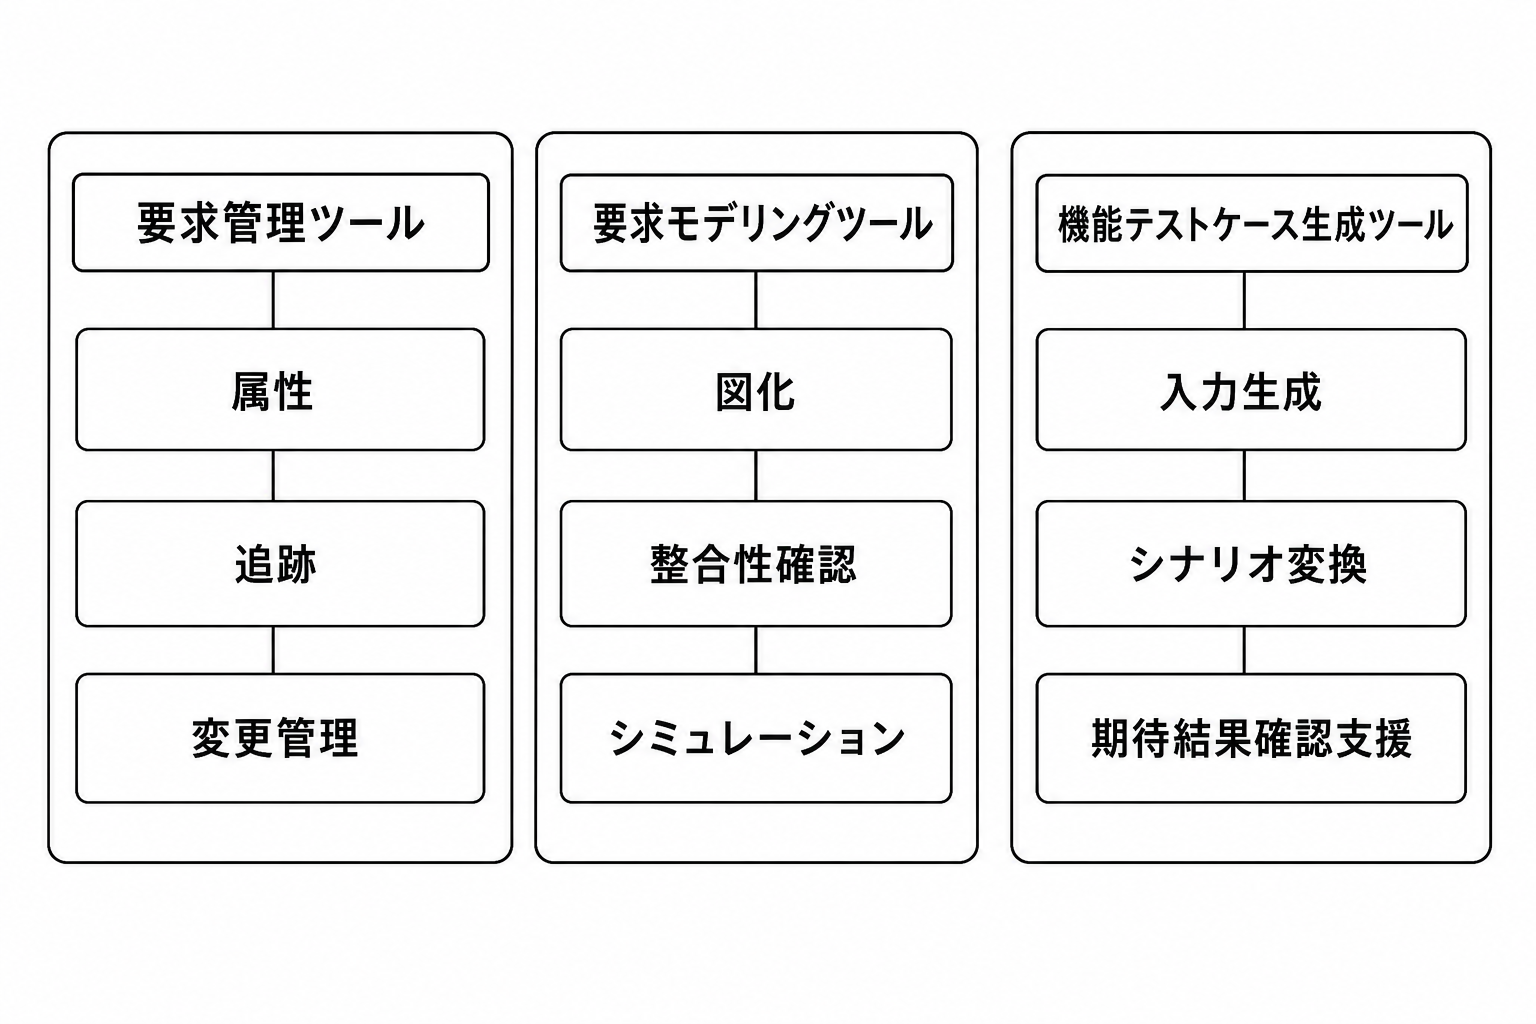
\includegraphics[width=0.96\linewidth]{assets/generated_figures/ch01/fig-ch01-12.png}}{\fbox{\parbox[c][48mm][c]{0.9\linewidth}{\centering 画像生成待ち\\要求ツールの分類図}}}
\par\smallskip
\refstepcounter{figure}\label{fig:ch01-12}図 \thefigure: 要求ツールの分類図
\end{center}
図 \thefigure は、要求ツールの分類図を視覚的に整理したものである。
\par\smallskip
